\documentclass[a4paper]{article}

\usepackage{tikz}
\usepackage{graphicx}
%\usepackage{subfig}
\usepackage{algorithmicx}
\usepackage{float}
\usepackage{caption}
\usepackage{subcaption}
\usepackage{amsmath}
\usepackage{hyperref}


\def\N{\mathbb{N}} % mnozica naravnih stevil
\def\Z{\mathbb{Z}} % mnozica celih stevil
\def\Q{\mathbb{Q}} % mnozica racionalnih stevil
\def\R{\mathbb{R}} % mnozica realnih stevil
\def\C{\mathbb{C}} % mnozica kompleksnih stevil
\def\D{\mathbb{D}} % enotski disk
\def\H{\mathbb{H}} % zgornja polravnina
\def\K{\mathbb{K}} % Polje 
\newcommand{\geslo}[2]{\noindent\textbf{#1} \quad \hangindent=1cm #2\\[-1pc]}

\def\qed{$\hfill\Box$}   % konec dokaza
\def\qedm{\qquad\Box}   % konec dokaza v matematičnem načinu
\newtheorem{izrek}{Izrek}
\newtheorem{trditev}{Trditev}
\newtheorem{posledica}{Posledica}
\newtheorem{lema}{Lema}
\newtheorem{pripomba}{Pripomba}
\newtheorem{definicija}{Definicija}
\newtheorem{zgled}{Zgled}

\title{}

\begin{document}
%%%%%%%%%%%%%%%%%%%%%%%%%%%%%%%%%%%%%%%%%%%%%%%%%%%%%%%%%%%%%%%%%%%%%
\maketitle
%%%%%%%%%%%%%%%%%%%%%%%%%%%%%%%%%%%%%%%%%%%%%%%%%%%%%%%%%%%%%%%%%%%%%

Testirali smo dve metodi za reševanje problema. Prva metoda je bila bisekcijska metoda, druga pa požrešna metoda. Spreminjali smo tako $n$ kot $p$ parameter. Pri vsakem paru parametrov smo poskus ponovili za $100$ različnih problemov. Problem sestoji iz matrike razdalji, ki je velikosti $n \times n$ in parametra $p$, ki nam pove koliko lokacij si bomo izbrali. Matrike so bile naključno generirane, pri čemer smo upoštevali tudi trikotniško neenakost. Da je poskus ponovljiv smo tudi fiksirali random seed in sicer z $np.random.seed(2022)$. Ker se bisekcija metoda lahko zacikla, smo jo omejili, da se po $200$ ne uspelih poskusih samostojno prekine in vrne $None$, kar pomeni, da metoda ni skonvergirala. 

\section{$n = 10$}
Najprej smo testirali pri $n = 10$. Ker imamo tukaj opravka še z razmeroma malimi matrikami, smo izvedli poskus za $p \in \{3, 4, 5, 6, 7\}$. Pri vsakem poskusu smo si zapisali najmanjšo razdaljo med točkami, par točk pri katerih je ta razdalja dosežena, množico vseh točk, ki jih imamo v izboru in čas izvajanja. Zanima nas predvsem katera metoda se je boljše odrezala. 

\begin{figure}[h]
	\begin{subfigure}[t]{0.45\textwidth}
		\centering
		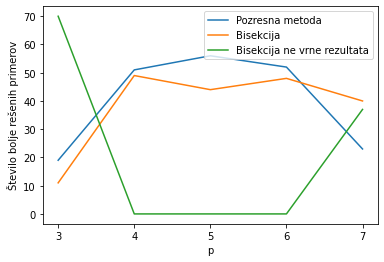
\includegraphics[width=\textwidth]{n_10.png}
		\caption{Uspešnost posamezne metode pri $n = 10$}
		\label{n_10_count}
	\end{subfigure}
	\hfill
	\begin{subfigure}[t]{0.45\textwidth}
		\centering
		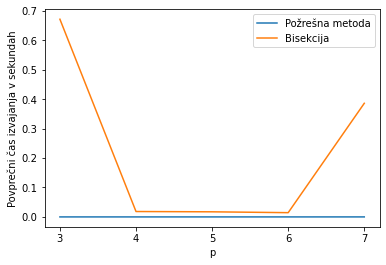
\includegraphics[width=\textwidth]{n_10_time.png}
		\caption{Povprečen čas izvajanja metode pri različnih $p$ in $n = 10$}
		\label{n_10_time}
	\end{subfigure}
    \caption{Rezultati pri $n = 10$.}
    \label{fig:n_10}
\end{figure}


Iz grafa je razvidno, da je bila bisekcija metoda pri $p = 3$ in $p = 7$ večkrat neuspešna in ni skonvergirala, medtem ko je pri $p \in \{4, 5, 6\}$ bila uspešna vsakič. 
Pri primerjavi dobljenih rezultatih je pri $p \in \{3, 4, 5, 6\}$ bila uspešnejša požrešna metoda, medtem ko se je to spremenilo pri $p = 7$, kjer je kljub neskonvergiranim vrednostim bila še vedno boljša bisekcijska metoda. 

Pogledali smo si tudi čas izvajanja posamezne metode. 

Vemo, da v primerih $p = 3$ in $p = 7$ metoda ni skonvergirala, torej je tam očitno čas izvajanja večji. Pri ostalih $p$ pa je čas izvajanja pri obeh metodah primerljiv.

\section{$n = 20$}
Nadalje smo testirali metodo pri $n = 20$. Poskus smo najprej ponovili za $p \in \{5, 10, 15\}$, ker pa sta metodi dobro konvergirali, smo dodali še dva parametra, tako da smo si pogledali pri $p \in \{5, 8, 10, 12, 15\}$. Tudi tukaj smo si pogledali, kako uspešna je posamezna metoda. 

\begin{figure}[h]
	\begin{subfigure}[t]{0.45\textwidth}
		\centering
		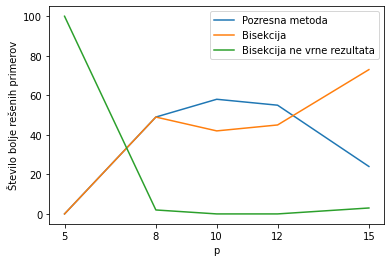
\includegraphics[width=\textwidth]{n_20.png}
		\caption{Uspešnost posamezne metode pri $n = 20$l}
		\label{n_20_count}
	\end{subfigure}
	\hfill
	\begin{subfigure}[t]{0.45\textwidth}
		\centering
		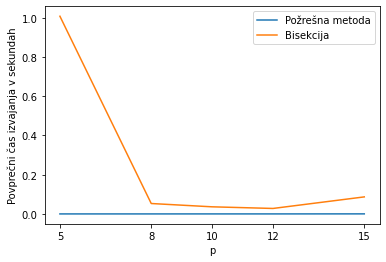
\includegraphics[width=\textwidth]{n_20_time.png}
		\caption{Povprečen čas izvajanja metode pri različnih $p$ in $n = 20$}
		\label{n_20_time}
	\end{subfigure}
    \caption{Rezultati pri $n = 20$.}
    \label{fig:n_20}
\end{figure}

Bisekcijska metoda spet ni skonvergirala za najmanjši $p$, je pa bila z večanjem $p$ čedalje bolj uspešna. Pri $p \in \{5, 8, 10, 12\}$ je spet prevladovala požrešna metoda, pri $p = 15$, pa se je za bistveno boljšo izkazala bisekcijska metoda, čeprav parkrat vseeno ni skonvergirala. 

Tudi v tem primeru ne moremo primerjati časa izvajanja metode pri najmanjšem $p = 5$, saj bisekcijska metoda tudi tukaj ni skonvergirala. Pri ostalih $p$ pa vidimo da je čas izvajanja spet primerljiv, pri čemer pa se za največji $p = 15$ začne čas že povečevati, je pa ta sprememba še vedno sprejemljiva.

\section{$n = 50$}
Nazadnje smo pogledali še $n = 50$. Tukaj smo si prav tako najprej zastavili $3$ parametre $p$ in sicer $p \in \{10, 25, 40\}$. Čas izvajanja je bil še sprejemljiv, tako da smo tudi tokrat povečali množico parametrov, tako da smo si ogledali za $p \in \{10, 20, 25, 30, 40\}$. 

\begin{figure}[h]
	\begin{subfigure}[t]{0.45\textwidth}
		\centering
		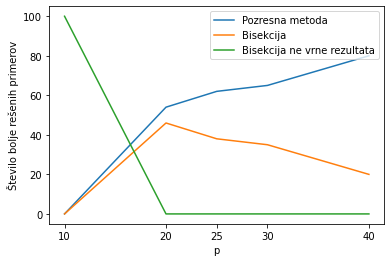
\includegraphics[width=\textwidth]{n_50.png}
		\caption{Uspešnost posamezne metode pri $n = 50$}
		\label{n_50_count}
	\end{subfigure}
	\hfill
	\begin{subfigure}[t]{0.45\textwidth}
		\centering
		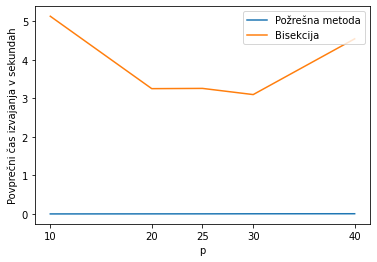
\includegraphics[width=\textwidth]{n_50_time.png}
		\caption{Povprečen čas izvajanja metode pri različnih $p$ in $n = 50$}
		\label{n_50_time}
	\end{subfigure}
    \caption{Rezultati pri $n = 50$.}
    \label{fig:n_50}
\end{figure}

Tako kot v prejšnjih primerih tudi tokrat bisekcijska metoda ni skonvergirala za najmanjši $p$. Se je pa v primerjavi s prejšnjimi primeri njena uspešnost tokrat slabšala. Požrešna metoda je bila tukaj za vse $p$ bolj uspešna.

Tudi z vidika časovne zahtevnosti, se je požrešna metoda izkazala za bistveno boljšo. Povprečni čas izvajanja z bisekcijsko metodo, je bil namreč za kar par sekund počasnejši kot čas izvajanja požrešne metode. Glede na rezultate bisekcije metode z počasnejšim in zahtevnejšim algoritmom nismo pridobili boljšega rezultata. 

\end{document}

